\documentclass[tikz,border=2pt]{standalone}
\usepackage{amsmath}
\usetikzlibrary{arrows.meta,decorations.pathreplacing}
\begin{document}
% Step j = 2 for a_1 = (1,1,0)^T, a_2 = (1,0,1)^T, drawn in the plane span{a_1, a_2} (true lengths):
% v_1 = a_1 (length sqrt 2), the projection of a_2 onto v_1 is (1/2)v_1, and v_2 = a_2 - (1/2)v_1 is
% perpendicular to v_1 (length sqrt(3/2)).
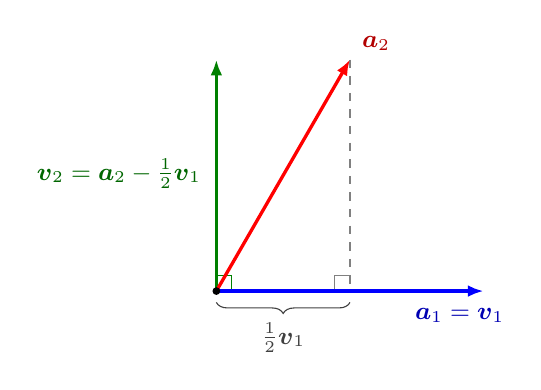
\begin{tikzpicture}[font=\small, >={Latex[length=2mm]}, x=2.4cm, y=2.4cm]
  % a_1 = sqrt2 q_1, a_2 = (1/sqrt2) q_1 + sqrt(3/2) q_2 in plane coordinates
  \coordinate (O) at (0,0);
  \coordinate (A1) at (1.4142,0);
  \coordinate (A2) at (0.7071,1.2247);
  \coordinate (P) at (0.7071,0);
  \coordinate (V2) at (0,1.2247);
  % projection: perpendicular from a_2 to the line of v_1
  \draw[gray, thick, dashed] (A2) -- (P);
  \draw[gray] (0.7071,0.08) -- (0.6271,0.08) -- (0.6271,0);
  \draw[decorate, decoration={brace, mirror, amplitude=4pt}, gray!50!black] (0,-0.06) -- (0.7071,-0.06)
    node[midway, below=4pt] {$\tfrac12\boldsymbol{v}_1$};
  % v_2 = a_2 - (1/2) v_1, parallel copy from the foot and the result from the origin
  \draw[->, green!50!black, very thick] (O) -- (V2);
  \node[green!40!black, anchor=east] at (-0.03,0.62) {$\boldsymbol{v}_2=\boldsymbol{a}_2-\tfrac12\boldsymbol{v}_1$};
  \draw[green!50!black] (0.08,0) -- (0.08,0.08) -- (0,0.08);
  % inputs
  \draw[->, blue, very thick] (O) -- (A1);
  \node[blue!70!black, anchor=north west] at (1.0,-0.04) {$\boldsymbol{a}_1=\boldsymbol{v}_1$};
  \draw[->, red, very thick] (O) -- (A2);
  \node[red!70!black, anchor=south west] at (0.72,1.22) {$\boldsymbol{a}_2$};
  \fill (O) circle (1.4pt);
\end{tikzpicture}
\end{document}
